\section{Aufgabe 2}
\label{sec:Aufgabe2}
% \lstinputlisting[language=Python, firstline=15, lastline=21]{plots/plot.py}
Teilaufgabe a) und b) sind auf einem seperaten Zettel abgegeben worden.
Für die Berechnung des Informationsgewinns in Abhängigkeit verschiedener
Schnitte wurden zunächst Schnitte gewählt, bei denen immer noch ein Wert der
Tabelle über dem größen Schnittwert und ein Wert unter dem geringsten liegt.
Die gewählten Schnitte für die drei verbleibenden sind :
\begin{align*}
  Cut_{\text{Temperatur}}&=[19, 20, 21, 22, 23, 24, 25, 26, 27, 28]\\
  Cut_{\text{Vorhersage}}&=[0.5, 1.5]\\
  Cut_{\text{Feuchtigkeit}}&=[70, 72, 74, 76, 78, 80, 82, 84, 86, 88, 90]
\end{align*}
In Abhängigkeit dieser Cuts wurden, wie in der handschriftlichen Abgabe beispielhalft
durchgegeführt, der Informationsgewinn geberechnet. In Abbildung \ref{fig:IG} sind
die Informationsgewinne für die einzelnen Cuts dargestellt.
\begin{figure}[h]
  \centering
  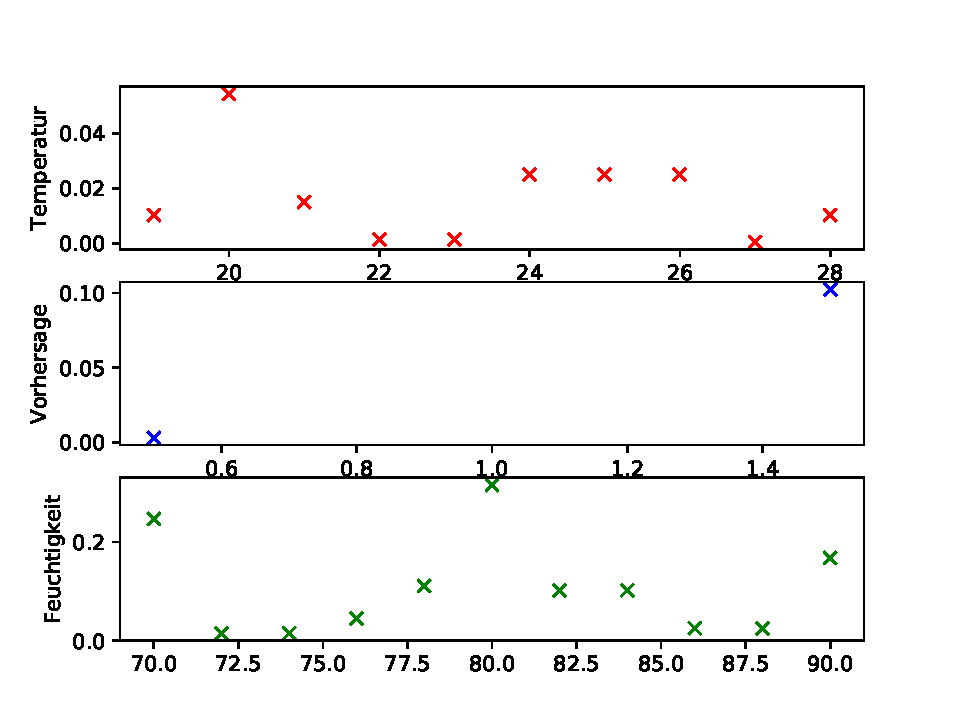
\includegraphics[height = 8cm]{plots/Informationsgewinn.pdf}
  \caption{Informationsgewinn in Abhängigkeit der Cuts für die einzelnen
           Attribute.}
  \label{fig:IG}
\end{figure}
Die größten Werte für die drei Attribute sind:
\begin{align*}
  IG_{\text{Temperatur}}&=0.0544\\
  IG_{\text{Vorhersage}}&=0.1022\\
  IG_{\text{Feuchtigkeit}}&=0.3149
\end{align*}
Demnach lohnt es sich am meisten das Attribut Feuchtigkeit zu verwenden um
die Daten zu trennen.
